% ---------------------------------------------------------------------------
% dendritic_credit_workshop_appendix.tex — backup slides (7 frames).
% The seven strongest backup frames kept in the single-deck build: adjoint
% chain, U(M) derivation + caveat, factorial control battery, validity /
% clean-agreement audit, reliability + same-span, CIFAR-10 confirmation,
% references. The five
% frames cut in the one-deck revision are preserved verbatim in the
% \iffalse block at the end of this file (nothing is lost).
% Backup frames keep the boxed \eqpanel look by design.
% ---------------------------------------------------------------------------

% A1 — adjoint chain
\begin{frame}{Appendix: the adjoint chain, from implicit function to path product}
  \begin{columns}[T,onlytextwidth]
    \begin{column}{0.55\textwidth}
      \eqpanel[general adjoint]{%
        \small
        \[
          \bm F(\bm V,\bm g,\bm x)=\bm 0,\qquad
          J_V=\frac{\partial\bm F}{\partial\bm V},\qquad
          J_V^{\mathsf T}\bm q=\nabla_{\bm V}\mathcal L
        \]
        \[
          \frac{\partial\mathcal L}{\partial g_i}
          =-\bm q^{\mathsf T}\frac{\partial\bm F}{\partial g_i}
          =x_i(E_i-V_n)\,q_n
        \]
        {\scriptsize\color{Mute}synapse-local factor $\times$ compartment
         adjoint\par}}
      {\footnotesize With the residual convention $\bm F=G\bm V-\bm b$.
       For the triangular tree system,
       $q_n=R_n^{\mathrm{tot}}\,\partial\mathcal L/\partial V_n$, so the
       adjoint and compartment factorizations are the same identity with the
       input-resistance factor moved between terms.\par}
    \end{column}
    \begin{column}{0.42\textwidth}
      {\footnotesize In a reciprocal passive cable, $J_V=G$ is symmetric
       positive definite and $G^{-\mathsf T}=G^{-1}$: the adjoint is a
       Green's-function solve. For a general nonsymmetric or recurrent
       compartmental system the inverse transpose is essential.\par
       \vspace{0.10cm}
       This fixed-point adjoint is the steady-state member of the
       Almeida--Pineda recurrent-backpropagation lineage.\par}
    \end{column}
  \end{columns}
  \vfill
  \takeaway{Credit is always eligibility times an adjoint; only the adjoint changes.}
  \vspace{0.04cm}
\end{frame}

% A2 — U(M) derivation
\begin{frame}{Appendix: deriving $U(M)$ and its exactness caveat}
  \begin{columns}[T,onlytextwidth]
    \begin{column}{0.55\textwidth}
      \eqpanel[descent lemma]{%
        \small For $L$-Lipschitz $\nabla\mathcal L$ and
        $\bm w^{+}=\bm w-\eta M\widehat{\bm g}$, $\widehat{\bm g}=\bm g+\bm\xi$:
        \[
          \begin{aligned}
            \E\,\mathcal L(\bm w^{+})\leq{}&\mathcal L(\bm w)
              -\eta\,\bm g^{\mathsf T}M\bm g\\
            &+\frac{L\eta^{2}}{2}
              \bigl(\lVert M\bm g\rVert_2^{2}+\tr(M\Sigma M^{\mathsf T})\bigr)
          \end{aligned}
        \]
        Optimizing the right side over $\eta$ when
        $\bm g^{\mathsf T}M\bm g>0$:
        \[
          U(M)=\frac{[\bm g^{\mathsf T}M\bm g]^{2}}
            {2L\bigl\{\lVert M\bm g\rVert_2^{2}
              +\tr(M\Sigma M^{\mathsf T})\bigr\}}
        \]}
    \end{column}
    \begin{column}{0.42\textwidth}
      {\footnotesize\deftag{caveat}\par
       The bound is an upper guarantee for a general $L$-smooth loss and is
       exact for the corresponding quadratic when curvature equals $L$ on the
       update directions; comparisons of $U(M)$ otherwise order guarantees,
       not necessarily realized losses.\par
       \vspace{0.10cm}
       Diagnostics: $U(M)$ predicted norm-matched one-step progress with
       Spearman $\rho=0.937$ and final held-out accuracy with $\rho=0.916$
       across 540 dendritic-route conditions; spectral capture alone
       predicted one-step progress at $\rho=0.877$.\par}
    \end{column}
  \end{columns}
  \vfill
  \takeaway{One-step geometry predicts within-family progress; trajectory-accrued advantages can escape it.}
  \vspace{0.04cm}
\end{frame}

% A3 — factorial control battery
\begin{frame}{Appendix: factorial control battery and implementation equivalence}
  \begin{columns}[T,onlytextwidth]
    \begin{column}{0.60\textwidth}
      \centering
      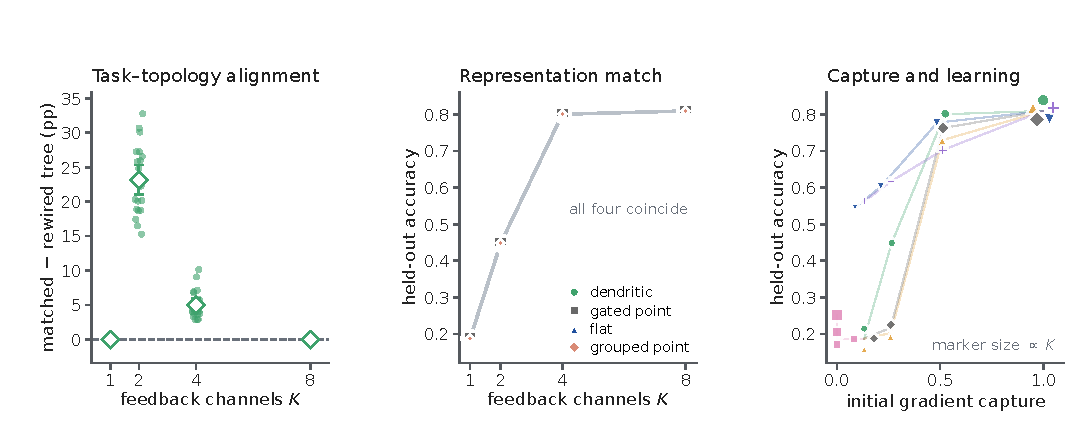
\includegraphics[width=\linewidth,height=4.30cm,keepaspectratio]{pdf_assets/factorial_controls_legend.pdf}
    \end{column}
    \begin{column}{0.36\textwidth}
      \footnotesize
      \deftag{topology alignment}\par matched tree minus rewired tree:
      $+0.231$ at $K{=}2$, $+0.050$ at $K{=}4$; 20/20 paired seeds each.\par
      \vspace{0.10cm}
      \deftag{representation match}\par dendritic, gated-point, flat and
      grouped-point implementations coincide exactly (maximum accuracy
      difference 0) when given identical routed fields.\par
      \vspace{0.10cm}
      \deftag{capture is not fate}\par fields with similar initial capture
      but different route signs and task alignment learned differently.\par
    \end{column}
  \end{columns}
  \vfill
  \takeaway{An address resource any point system can buy with the same routes.}
  \vspace{0.04cm}
\end{frame}

% A4 — validity audit + clean agreement
\begin{frame}{Appendix: input-validity audit and clean exact/BP agreement}
  \begin{columns}[T,onlytextwidth]
    \begin{column}{0.55\textwidth}
      \footnotesize
      \deftag{outcome-independent rule}\par signed synthetic drive is invalid
      for a positive-conductance shunting denominator: 640 signed-shunting
      runs are invalid, and the 400-run inhibitory-dose family that depends
      on them is excluded with its 200 valid partners --- 840 of 1,840 runs
      leave inference; all remain in the ledger.\par
      \vspace{0.10cm}
      \deftag{clean-source audit}\par all 320 detached clean-source runs
      passed the configuration, log, metric and checkpoint audit; synthetic
      shunting uses a non-negative transfer.\par
      \vspace{0.10cm}
      \deftag{agreement}\par all four depth-averaged exact-minus-BP intervals
      include zero; mean across 160 pairs $-0.055$ pp; largest single pair
      difference $5.90$ pp.\par
    \end{column}
    \begin{column}{0.41\textwidth}
      \centering
      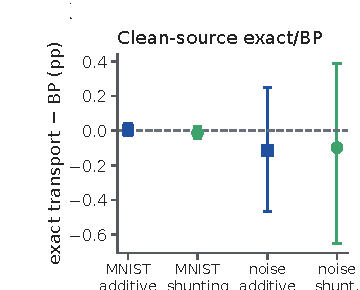
\includegraphics[width=\linewidth,height=3.55cm,keepaspectratio]{pdf_assets/clean_agreement.pdf}\par
      {\scriptsize\color{Mute}10 seeds $\times$ 4 depths $\times$ 2 tasks
       $\times$ 2 cores $\times$ 2 methods --- condition-average agreement,
       not pointwise identity\par}
    \end{column}
  \end{columns}
  \vfill
  \takeaway{The clean audit supports agreement on average, never formal equivalence.}
  \vspace{0.04cm}
\end{frame}

% A5 — reliability gain + same-span conditioning
\begin{frame}{Appendix: reliability gain, and same-span conditioning}
  \begin{columns}[T,onlytextwidth]
    \begin{column}{0.485\textwidth}
      \eqpanel[finite-step gain]{%
        \small For disjoint branches with signal $S_b$, noise $N_b$, step
        $\eta=c/L$:
        \[
          \mathcal G_c(\bm a)=\frac{c}{L}\sum_b
            \Bigl[a_bS_b-\frac{c\,a_b^{2}}{2}(S_b+N_b)\Bigr]
        \]
        \[
          a_b^{*}=\min\Bigl\{1,\frac{S_b}{c\,(S_b+N_b)}\Bigr\}
        \]}
      {\footnotesize A point model supplied with identical branch gates must
       match --- and did, to numerical precision.\par
       {\scriptsize\color{Mute}trained branch model, 50 fresh seeds: aligned
        shunting beat the best global gain by $0.001817$ in one-step loss
        reduction (49/50); final aligned-minus-no-shunt loss was null
        ($0.000425$, $P=0.154$)\par}}
    \end{column}
    \begin{column}{0.485\textwidth}
      \eqpanel[same-span field iteration]{%
        \small
        \[
          \bm f_{t+1}=\bm f_t-cA(\bm f_t-\bm g-\bm\xi_t)
        \]
        \[
          \E\,\mathcal L_T=\frac12\sum_j
            \Bigl[B_{j,T}+\frac{\sigma^{2}}{n}V_{j,T}\Bigr]
        \]}
      \centering
      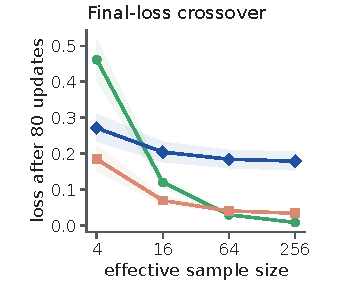
\includegraphics[height=2.00cm,keepaspectratio]{pdf_assets/same_span_crossover_e.pdf}\par
      {\scriptsize\color{Mute}\raggedright rank-eight same-span coordinates,
       condition numbers 1 / 15 / 388.5: slow modes filter noise at small
       $n$, orthogonal modes cut bias at large $n$; predicted crossovers
       $n^{*}=38.5$, $8.25$\par}
    \end{column}
  \end{columns}
  \vfill
  \takeaway{Conductance realizes the predicted ordering; conditioning trades bias against variance.}
  \vspace{0.04cm}
\end{frame}

% A6 — fresh CIFAR-10 confirmation
\begin{frame}{Appendix: harder data isolates the feedback bottleneck}
  \framesubtitle{Fresh 20-seed raw-additive confirmation; flattened CIFAR-10 is a transfer assay, not a vision benchmark.}
  \begin{columns}[T,onlytextwidth]
    \begin{column}{0.56\textwidth}
      \centering
      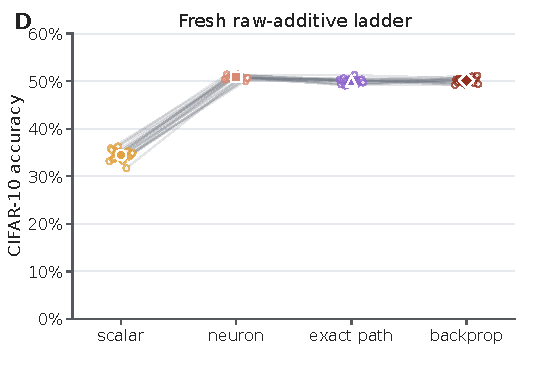
\includegraphics[width=\linewidth,height=4.75cm,keepaspectratio]{pdf_assets/cifar_confirmatory_ladder.pdf}\par
      {\scriptsize\color{Mute}Gray lines pair seeds; large symbols show means
       and 95\% intervals.\par}
    \end{column}
    \begin{column}{0.40\textwidth}
      \footnotesize
      \deftag{adequate control}\par matched BP: \(50.12\%\); all 80 fits passed
      source, calibration, checkpoint and convergence audits.\par
      \vspace{0.12cm}
      \deftag{neuron identity}\par \(+16.39\) pp over strict scalar
      (95\% CI 15.88--16.91; 20/20 seeds).\par
      \vspace{0.12cm}
      \deftag{path boundary}\par exact path was \(0.86\) pp below
      neuron-specific feedback; the prespecified path-resolution gate failed.\par
      \vspace{0.12cm}
      \deftag{implementation check}\par exact path was equivalent to matched BP
      within \(\pm1\) pp (TOST \(P=1.58\times10^{-5}\)).\par
    \end{column}
  \end{columns}
  \vfill
  \takeaway{Harder data magnifies neuron identity, not a generic benefit of finer dendritic transport.}
  \vspace{0.04cm}
\end{frame}

% A7 — references
\begin{frame}{Appendix: references}
  \vspace{0.05cm}
  \begin{columns}[T,onlytextwidth]
    \begin{column}{0.48\textwidth}
      % ragged right + tied journal~year units: no orphaned years
      {\color{Mute}\fontsize{7}{9}\selectfont\raggedright
       Rumelhart, Hinton \& Williams, \emph{Nature}~1986.\par
       Rall, dendritic cable theory, 1962.\par
       Almeida 1987; Pineda 1987 --- recurrent backpropagation.\par
       Werfel, Xie \& Seung, \emph{Neural Computation}~2005.\par
       Lillicrap, Cownden, Tweed \& Akerman, \emph{Nat.~Commun.}~2016.\par
       N\o kland, \emph{NeurIPS}~2016.\par
       Fr\'emaux \& Gerstner, \emph{Front.~Neural Circuits}~2016.\par
       Scellier \& Bengio, \emph{Front.~Comput.~Neurosci.}~2017.\par
       Whittington \& Bogacz, \emph{Neural Computation}~2017.\par
       Guerguiev, Lillicrap \& Richards, \emph{eLife}~2017.\par
       Sacramento, Costa, Bengio \& Senn, \emph{NeurIPS}~2018.\par
       Payeur, Guerguiev, Zenke, Richards \& Naud,
         \emph{Nat.~Neurosci.}~2021.\par
       Song et al., inferred-activity plasticity, 2024.\par}
    \end{column}
    \begin{column}{0.48\textwidth}
      {\color{Mute}\fontsize{7}{9}\selectfont\raggedright
       Holt \& Koch, shunting and firing rates, \emph{Neural Comput.}~1997.\par
       Chance, Abbott \& Reyes, gain modulation, \emph{Neuron}~2002.\par
       Destexhe, Rudolph \& Par\'e, high-conductance state,
         \emph{Nat.~Rev.~Neurosci.}~2003.\par
       Vogels et al., inhibitory plasticity, \emph{Science}~2011.\par
       Gidon \& Segev, spatial inhibitory domains, \emph{Neuron}~2012.\par
       Lovett-Barron et al., dendritic inhibition,
         \emph{Nat.~Neurosci.}~2012.\par
       Carandini \& Heeger, divisive normalization,
         \emph{Nat.~Rev.~Neurosci.}~2012.\par
       Jordan et al., conductance-based dendrites, 2024.\par
       MICrONS Consortium, \emph{Nature}~2025.\par
       Schneider-Mizell et al., inhibitory census, \emph{Nature}~2025.\par
       Ding et al., like-to-like wiring, \emph{Nature}~2025.\par
       Francioni et al., vectorized instructive signals,
         \emph{Nature}~2026.\par
       Safaai, Richards \& Sabatini, local credit manuscript, 2026.\par}
    \end{column}
  \end{columns}
  \vfill
  \takeaway{All quantitative claims trace to the journal manuscript and its source-data package.}
  \vspace{0.04cm}
\end{frame}

% ===========================================================================
% CUT FRAMES — preserved, not compiled.
% The five backup frames removed in the one-deck revision (former A2
% quotient-rule steps, A4 weighted projection / Ky--Fan, A5 reliability gain
% physical test, A6 Sherman--Morrison selectivity, A9 same-span
% bias--variance, A10 full-tree all-scan boundary; A5+A9 were merged into
% the kept "reliability + same-span" frame above). To restore one, move it
% above this block.
% ===========================================================================
\iffalse

% former A2 — quotient rule steps
\begin{frame}{Appendix: quotient-rule steps for eligibility}
  \begin{columns}[T,onlytextwidth]
    \begin{column}{0.52\textwidth}
      \eqpanel[synaptic conductance]{%
        \small With $V_n=N_n/G_n$,\quad
        $\partial_{g_i}N_n=x_iE_i$, \ $\partial_{g_i}G_n=x_i$:
        \[
          \begin{aligned}
            \partial_{g_i}V_n
            &=\partial_{g_i}\bigl(N_nG_n^{-1}\bigr)
             =x_iE_iG_n^{-1}-N_nG_n^{-2}x_i\\
            &=x_iG_n^{-1}\bigl(E_i-N_nG_n^{-1}\bigr)
             =x_iR_n^{\mathrm{tot}}(E_i-V_n)
          \end{aligned}
        \]}
    \end{column}
    \begin{column}{0.44\textwidth}
      \eqpanel[coupling conductance]{%
        \small The same algebra for a child coupling:
        \[
          \frac{\partial V_n}{\partial g^{\mathrm{den}}_{c\to n}}
          =R_n^{\mathrm{tot}}\bigl(f_c(V_c)-V_n\bigr)
        \]}
      {\footnotesize The driving-force form is exact for any conductance that
       enters both numerator and denominator. If $g_i=\psi(\theta_i)$, then
       $\partial_{\theta_i}\mathcal L
        =(\partial_{g_i}\mathcal L)\,\psi'(\theta_i)$.\par}
    \end{column}
  \end{columns}
  \vfill
  \takeaway{Every conductance parameter of the tree has a closed-form, synapse-local sensitivity.}
  \vspace{0.04cm}
\end{frame}

% former A4 — weighted projection and Ky-Fan
\begin{frame}{Appendix: weighted projection, covariance matching, Ky--Fan}
  \begin{columns}[T,onlytextwidth]
    \begin{column}{0.52\textwidth}
      \eqpanel[weighted projection]{%
        \small
        \[
          \bar{\bm w}=W^{-1/2}\bm w,\quad
          \bar{\bm g}=W^{1/2}\bm g,\quad
          \overline\Phi=W^{1/2}\Phi_{T,K}
        \]
        \[
          \bm z^{*}=\overline\Phi^{\dagger}\bar{\bm g},\qquad
          P_{\Phi}=\overline\Phi\,\overline\Phi^{\dagger},\qquad
          \mathcal C_K=\frac{\bar{\bm g}^{\mathsf T}P_{\Phi}\bar{\bm g}}
            {\bar{\bm g}^{\mathsf T}\bar{\bm g}}
        \]}
      \eqpanel[covariance matching]{%
        \small
        \[
          \frac{\E\lVert P_{\Phi}\bar{\bm g}\rVert^{2}}
               {\E\lVert\bar{\bm g}\rVert^{2}}
          =\frac{\tr(P_{\Phi}\overline C_g)}{\tr(\overline C_g)}
        \]
        {\scriptsize\color{Mute}$\overline C_g=\E[\bar{\bm g}\bar{\bm g}
         ^{\mathsf T}]$; $W{=}I$ recovers the unweighted form.\par}}
    \end{column}
    \begin{column}{0.44\textwidth}
      {\footnotesize By the Ky--Fan principle, the unconstrained rank-$K$
       upper bound is the span of the leading $K$ eigenvectors of $C_g$.\par
       \vspace{0.10cm}
       The $K$-route ancestry span equals the span of the $K$ coarsest
       tree-Haar modes, so anatomy attains the rank-$K$ bound exactly when the
       leading rank-$K$ eigenspace lies inside the laminar span; its shortfall
       for a general covariance is bounded by the leading-eigenspace energy
       outside that span.\par
       \vspace{0.10cm}
       At $\eta=1/L_W$, projected and full one-step descent guarantees differ
       by exactly the factor $\mathcal C_K$.\par}
    \end{column}
  \end{columns}
  \vfill
  \takeaway{A route basis is useful only insofar as task-gradient energy lies in its span.}
  \vspace{0.04cm}
\end{frame}

% former A5 — reliability gain
\begin{frame}{Appendix: the reliability gain $a_b^{*}$, and its physical test}
  \begin{columns}[T,onlytextwidth]
    \begin{column}{0.50\textwidth}
      \eqpanel[finite-step gain]{%
        \small For disjoint branches with signal $S_b$, noise $N_b$, step
        $\eta=c/L$:
        \[
          \mathcal G_c(\bm a)=\frac{c}{L}\sum_b
            \Bigl[a_bS_b-\frac{c\,a_b^{2}}{2}(S_b+N_b)\Bigr]
        \]
        \[
          a_b^{*}=\min\Bigl\{1,\frac{S_b}{c\,(S_b+N_b)}\Bigr\}
        \]}
      {\footnotesize The reliability factor $S_b/(S_b+N_b)$ is the special
       case $c=1$. A point model supplied with identical branch gates must
       match --- and did, to numerical precision.\par}
    \end{column}
    \begin{column}{0.46\textwidth}
      \centering
      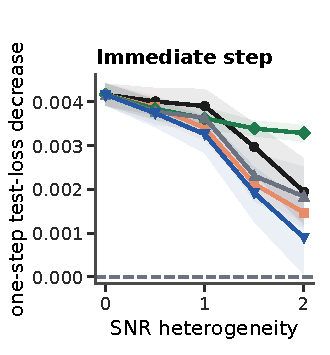
\includegraphics[height=3.15cm,keepaspectratio]{pdf_assets/reliability_step_c.pdf}\hspace{0.08cm}%
      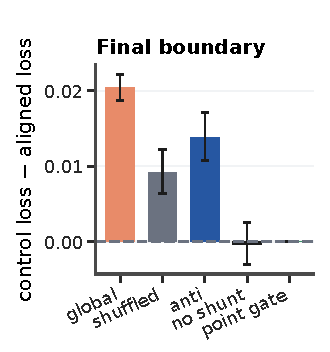
\includegraphics[height=3.15cm,keepaspectratio]{pdf_assets/reliability_final_f.pdf}\par
      \vspace{0.04cm}
      {\scriptsize\color{Mute}trained branch model, 50 fresh seeds: aligned
       shunting beat the best global gain by $0.001817$ in one-step loss
       reduction (49/50); final aligned-minus-no-shunt loss was null
       ($0.000425$, $P=0.154$)\par}
    \end{column}
  \end{columns}
  \vfill
  \takeaway{Conductance realizes the predicted ordering under a state clamp --- no more.}
  \vspace{0.04cm}
\end{frame}

% former A6 — Sherman-Morrison and selectivity
\begin{frame}{Appendix: Sherman--Morrison and electrotonic selectivity}
  \begin{columns}[T,onlytextwidth]
    \begin{column}{0.52\textwidth}
      \eqpanel[rank-one update]{%
        \small With $\bm q=G^{-1}\bm r$ and
        $G'=G+\kappa\,\bm e_k\bm e_k^{\mathsf T}$:
        \[
          (G+\kappa\,\bm e_k\bm e_k^{\mathsf T})^{-1}
          =G^{-1}-\frac{\kappa\,G^{-1}\bm e_k\bm e_k^{\mathsf T}G^{-1}}
            {1+\kappa\,\bm e_k^{\mathsf T}G^{-1}\bm e_k}
        \]
        \[
          \bm q'=\bm q-\frac{\kappa\,q_k}{1+\kappa\,(G^{-1})_{kk}}\,
            G^{-1}\bm e_k
        \]}
      {\footnotesize A current-matched additive perturbation changes $\bm b$
       but not $G$, so it cannot produce this adjoint update.\par}
    \end{column}
    \begin{column}{0.44\textwidth}
      \eqpanel[selectivity]{%
        \small With $\bm c_k=G^{-1}\bm e_k$, $r_k=(G^{-1})_{kk}$:
        \[
          \Delta\bm q=-a_k\bm c_k,\qquad
          |a_k|=\frac{\kappa_k|q_k|}{1+\kappa_kr_k}
        \]
        \[
          S_k=\frac{\operatorname{median}_{i\in D(k)}|c_{k,i}|}
                   {\operatorname{median}_{j\in C(k)}|c_{k,j}|}>1
        \]}
      {\footnotesize Dose sets amplitude (saturating at $|q_k|/r_k$); the
       Green's-function column sets spread. $S_k>1$ is necessary for
       descendant enrichment of absolute adjoint change, not sufficient for
       the full synaptic-gradient statistic.\par}
    \end{column}
  \end{columns}
  \vfill
  \takeaway{Input resistance controls dose response; axial and leak coupling control whether it is spatially selective.}
  \vspace{0.04cm}
\end{frame}

% former A9 — same-span bias-variance
\begin{frame}{Appendix: same-span conditioning trades bias against variance}
  \begin{columns}[T,onlytextwidth]
    \begin{column}{0.50\textwidth}
      \eqpanel[field iteration]{%
        \small
        \[
          \bm f_{t+1}=\bm f_t-cA(\bm f_t-\bm g-\bm\xi_t)
        \]
        For eigenmode $(\mu_j,\theta_j)$:
        \[
          \E\,\mathcal L_T=\frac12\sum_j
            \Bigl[B_{j,T}+\frac{\sigma^{2}}{n}V_{j,T}\Bigr]
        \]
        \[
          \begin{aligned}
            B_{j,T}&=(1-c\mu_j)^{2T}\theta_j^{2}\\
            V_{j,T}&=\frac{(c\mu_j)^{2}[1-(1-c\mu_j)^{2T}]}
              {1-(1-c\mu_j)^{2}}
          \end{aligned}
        \]}
    \end{column}
    \begin{column}{0.46\textwidth}
      \centering
      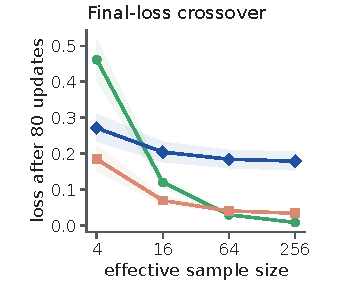
\includegraphics[height=2.85cm,keepaspectratio]{pdf_assets/same_span_crossover_e.pdf}\hspace{0.08cm}%
      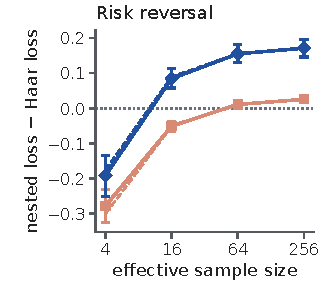
\includegraphics[height=2.85cm,keepaspectratio]{pdf_assets/same_span_risk_f.pdf}\par
      \vspace{0.04cm}
      {\scriptsize\color{Mute}three rank-eight same-span coordinates,
       condition numbers 1 / 15 / 388.5: slow modes filter noise at small
       $n$, orthogonal modes cut bias at large $n$; exact predicted median
       crossovers at $n^{*}=38.5$ and $8.25$\par}
    \end{column}
  \end{columns}
  \vfill
  \takeaway{Topology fixes capacity; conditioning trades bias against variance.}
  \vspace{0.04cm}
\end{frame}

% former A10 — full-tree all-scan boundary
\begin{frame}{Appendix: the full-tree all-scan boundary matches the predicted regime}
  \begin{columns}[T,onlytextwidth]
    \begin{column}{0.58\textwidth}
      \centering
      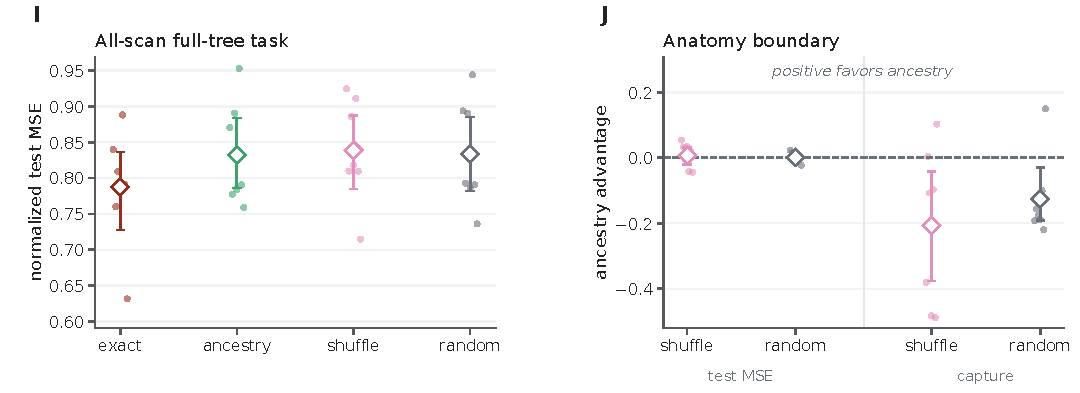
\includegraphics[width=\linewidth,height=3.90cm,keepaspectratio]{pdf_assets/fulltree_no_signed.pdf}
    \end{column}
    \begin{column}{0.38\textwidth}
      \footnotesize
      All 13 eligible scans, 520 method fits on complete reconstructed
      trees:\par
      \vspace{0.08cm}
      exact compartment error MSE \num{0.788}; topology $0.832$; random
      routes $0.833$; site-shuffled $0.839$ --- topology-minus-shuffle
      $0.0070$ $[-0.0207,0.0321]$: no reliable advantage.\par
      \vspace{0.08cm}
      In the coarse branch-surrogate family, a single channel already
      captured \num{0.965} of the measured response family's credit energy
      (effective rank 1.07), so every equal-rank dictionary spans it ---
      the regime where the credit-operator account predicts ties.\par
    \end{column}
  \end{columns}
  \vfill
  \takeaway{Rank-one task credit makes rank-matched dictionaries tie --- consistent with the predicted regime.}
  \vspace{0.04cm}
\end{frame}

\fi
